\section{Control Theoretic Model}
\label{sec:control}
Modeling the behavior of the workload in a computing infrastructure is challenging given the difficulties to non-linear identification techniques, the model uncertainty
generated by the complexity of the system as well as the multi-input multi-output (MIMO) nature of the system. Several alternatives have been presented to cover the main features of the workload in a computing infrastructure such as the fluid approximation model \cite{Malrait-2010}, or the approximation of the relation between the resource allocation and a given performance measure \cite{Padala-2009},\cite{Nathuji-2010}.

Optimal control is a common approach to calculate the resource allocation according to the actual workflow and the power consumption of the system  by minimizing a cost function. This minimization can be carried out by using partial derivatives \cite{Malrait-2010},\cite{Abdelzaher-SIGMETRICS-2008}, linear quadratic control (LQC) \cite{Padala-2009},\cite{Fu-FeBID-2009}, or by applying model predictive control (MPC) \cite{Nathuji-2010},\cite{Wang-2010}. The optimization problem consists of calculating a control input such that the cost of the control law is minimized while the required SLO of a set of applications is partially or completely reached.

\subsection{Model Estimation and Optimal Control}\label{workopcontrol}
In previous work \cite{Padala-2009},\cite{Abdelzaher-SIGMETRICS-2008}, the implemented control technique is composed of an online 
model estimator and a MIMO resource allocation controller as shown in Figure \ref{block}. The main goal of this controller is to optimally allocate the virtualized resources 
on a computing infrastructure so that the system can fulfill the required SLO. In current data center architectures, every tier of an application resides in a \emph{virtual machine} (VM) 
and a multi-tier application can run on several nodes. In this set up, several applications can be executed in one node, thus reducing the number 
of nodes in the computing infrastructure and minimizing costs.
\begin{figure}
\begin{center}
\begin{tabular}{c}
\scalebox{0.5}{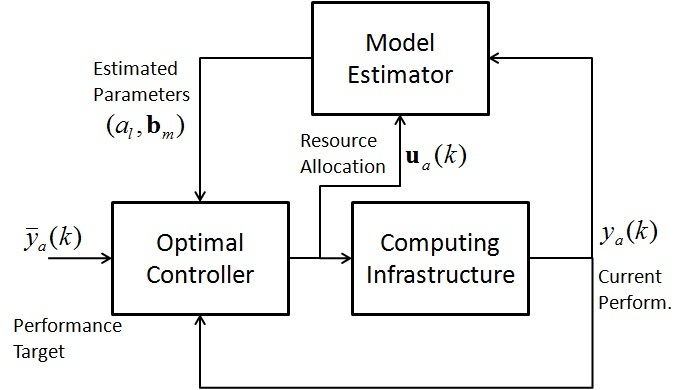
\includegraphics{block_model}}
\end{tabular}
\end{center}
\caption{Block diagram of the Optimal Controller with Model Estimator.}
\label{block}
\end{figure}

The model estimator uses an auto-regressive (AR) model to approximate the relation between the resource allocation of the application
$a \in A$, namely $\mathbf{u}_{a}(k) = \{ \mathbf{u}_{a,r,t}:r \in R, t \in T_{a} \}$ and the performance output $y_{a}(k)$ related to $a$. The AR model proposed in \cite{Abdelzaher-SIGMETRICS-2008} is given by,
\begin{eqnarray}
 y_{a}(k) &=& \sum_{l=1}^{n}a_{l}(k)y_{a}(k-l) \nonumber \\
& + & \sum_{m=0}^{n-1}\mathbf{b_{m}}^{T}(k)\mathbf{u}_{a}(k-m). \nonumber
\end{eqnarray}
We denote by $\mathbf{u}_{a,r,t}$ the actual allocation of the resource $r \in R$ for the application $a \in A$ in tier $t \in T_{a}$.
$A$ is the set of all hosted applications, $R$ is the set of all resource types considered and $T_{a}$ is the set of all tiers 
associated with application $a$. The scalar parameters $a_{l}(k)$ and the parameter vectors $\mathbf{b_{m}}(k)$ are estimated 
through a recursive least square (RLS) algorithm.
The optimizer searches for the required allocation vector ${\mathbf{\bar{u}}_{a}}$ that guarantees the performance target of the application $a$ while avoiding oscillations in 
resource allocation. This may be achieved by calculating $\mathbf{\bar{u}}_{a}$ that minimizes the following cost function,
\begin{equation}
 J_{a} = \left(y_{a}(k) - \bar{y}_{a}(k) \right)^{2} + q \| \mathbf{u}_{a}(k) - {\mathbf{u}_{a}}(k-1) \|^{2}.
\label{cost01}
\end{equation}
where $\bar{y}_{a}(k)$ is the desired performance associated with the application $a$. Note that the function $J_a$ is minimized for $\left(y_{a}(k) - \bar{y}_{a}(k) \right)^{2} \approx 0$
 leading the application $a$ to approach the desired performance. Furthermore (\ref{cost01}) is minimized if the difference 
$\| \mathbf{u}_{a}(k) - {\mathbf{u}_{a}}(k-1) \|$ becomes smaller, \emph{i.e.} when large changes in the resource allocation  during a sample period are avoided.
By solving $\frac{\partial J_{a}}{\partial{\mathbf{u}(k)}} = 0$ for $\mathbf{u}_{a}(k)$ the optimal control law for resource allocation is given by,
\begin{eqnarray}
 {\mathbf{\bar{u}}_{a}}(k) & = & ({\mathbf{b}_{0}\mathbf{b}_{0}}^{T} + qI)^{-1}\left[ \left(\bar{y}_{a}(k) - \sum_{l=1}^{n}a_{l}y_{a}(k-l)\right. \right. \nonumber \\
& & \left. \left.- \sum_{m=1}^{n-1}\mathbf{b}_{m}^{T}\mathbf{u}_{a}(k-m)\right)\mathbf{b_{0}} + q\mathbf{u}_{a}(k-1) \right], \nonumber
\end{eqnarray}
with $I$ the identity matrix and $q \in \Re$ a scaling factor. Note that, $a_i, b_j$ with $i=1,2,\cdots,n$, $j=0,1,2,\cdots,n-1$ are functions of $k$.


It might happen that the computing infrastructure cannot satisfy the resource allocation that has been calculated by the controller.
On that matter, Padala \emph{et. al.,} \cite{Padala-2009} present a complementary layer in the workload control called \emph{NodeController}. This module takes the resource 
allocation calculated by the optimal control (called \emph{AppController} in \cite{Padala-2009}) and, if the total requested allocation is less than the available 
capacity of the system, it assigns the resources as the optimal controller dictates. On the other hand, 
when the total resource allocation is higher than the available capacity we have  \emph{contention}. In such cases,
a new optimization problem is carried out in order to minimize the error between the required application performance and the 
actual one.

Padala \emph{et. al.,} \cite{Padala-2009} propose the following example. Two nodes, namely $n_{1}$ and $n_{2}$ hosting applications 1 and 2, sharing 
CPU and disk. Then, from application 1 we get the requests 
$\bar{u}_{1,cpu,web}$ and $\bar{u}_{1,disk,web}$.
Similarly, from application 2 we get the requests $\bar{u}_{2,cpu}$ and $\bar{u}_{2,disk}$.
Let us assume that node $n_{1}$ has enough capacity to fulfill the request for only one of the available resources. 
Modeling the shortage of resources we get $\Delta u_{1,r,web} = \bar{u}_{1,r,web}-u_{1,r,web}$ and 
$\Delta u_{2,r} = \bar{u}_{2,r}-u_{2,r}$. This problem is expressed in \cite{Padala-2009} as a constrained optimization problem,
\begin{eqnarray}
 \min J_{n1} & = & w_{1}\left(\frac{\partial y_{1}}{\partial u_{1,r,web}}\Delta u_{1,r,web} \right)^{2} \nonumber \\
 &&+
w_{2}\left(\frac{\partial y_{2}}{\partial u_{2,r}}\Delta u_{2,r} \right)^{2} \label{costn1} \\
\mbox{subject to} & & \nonumber \\
 \Delta u_{1,r,web} + \Delta u_{2,r} & \geq & \bar{u}_{1,r,web} + \bar{u}_{1,r,web} + \bar{u}_{2,r}-1 \nonumber \\
 \label{cond1} \\
\Delta u_{1,r,web} & \leq & 0, \label{cond2} \\
\Delta u_{2,r} & \leq & 0. \label{cond3}
\end{eqnarray}
where $\frac{\partial y_{1}}{\partial u_{1,r,web}}\Delta u_{1,r,web}$ estimates the error between the
requested and actual performance of application 1.
The condition in (\ref{cond1}) imposes a capacity constraint
that when violated means contention of one of the resources. The conditions given by (\ref{cond2}) and (\ref{cond3})
guarantee that no application can exceed its target performance to the detriment of the other.  
The weights $w_{1}$ and $w_{2}$ determine the priority of the applications, and the lower the weight, the greater the degradation.

Getting back to our example of Nimbus Cloud Corporation, we can map the SLAs to our actual control problem. Notice that the input of the system in Figure \ref{block}, corresponds to
the vector of required performance measurements for each application $a \in A$, then each entry of the vector is $\bar{y}_{a}(k)$. Let us assume that the outputs of the system
are \emph{uptime} $t_{u}$, \emph{latency} $\ell$ and \emph{abandon rate} $\alpha$, which are measurable. Latency is the time a server needs 
to process a request from the client. The Abandon rate of a server is the ratio between the rejected requests and the total number of received requests. 
Nimbus Cloud Corporation is able to assign 
the SLO values per application we require as a client and put them in the input array $\bar{y}_{a}(k)$. Since the values are fixed thresholds of performance, the indicator functions of 
performance are straightforward:

\begin{eqnarray}
&\left( (\ell \geq 300 ms) \land (\ell^{-1} \geq \frac{1}{650ms}) \right),& \nonumber \\
&\left(t_{u} \geq 95\%\right),& \nonumber \\
&\left(\alpha^{-1} \geq \frac{1}{10\%}\right).& \nonumber
\end{eqnarray}
Using the previous conditions the set of indicator functions will return \emph{true} if $300ms \leq \ell \leq 650ms$, similarly
 it will return \emph{true} if the minimum uptime is provided or the abandon rate is under the indicated threshold. Notice that other performance indices can be used such as
CPU utilization, memory usage or even the number of active processors in the computing infrastructure. Then, the SLOs and 
actually the SLIs are easily mapped into the depicted theoretical controls approach.